
\myNewSlide
\section*{Significantly different genealogy $\neq$ different phylogeny}
\begin{itemize}
    \item True ``gene tree'' can differ from true ``species tree'' for several biological reasons:
    \begin{itemize}
        \item deep coalescence,
        \item gene duplication/loss (you may be comparing paralogs),
        \item lateral gene transfer.
    \end{itemize}
\end{itemize}


\myNewSlide
\section*{There are lots of simulators out there}\large
\begin{itemize}
    \item Seq-gen, PAUP,  Indelible $\ldots$ - substitutions
    \item DAWG, Indelible $\ldots$ - alignment
    \item ms and multi-species coalescent simulators for within population samples
    \item Ginkgo, DIM SUM$\ldots$ biogeography simulators,
    \item $\ldots$
\end{itemize}
Parametric bootstrapping is very flexible and lots of tools are available.


\myNewSlide

{\Large You have to think about what sources of error are most relevant for {\bf your} data!}


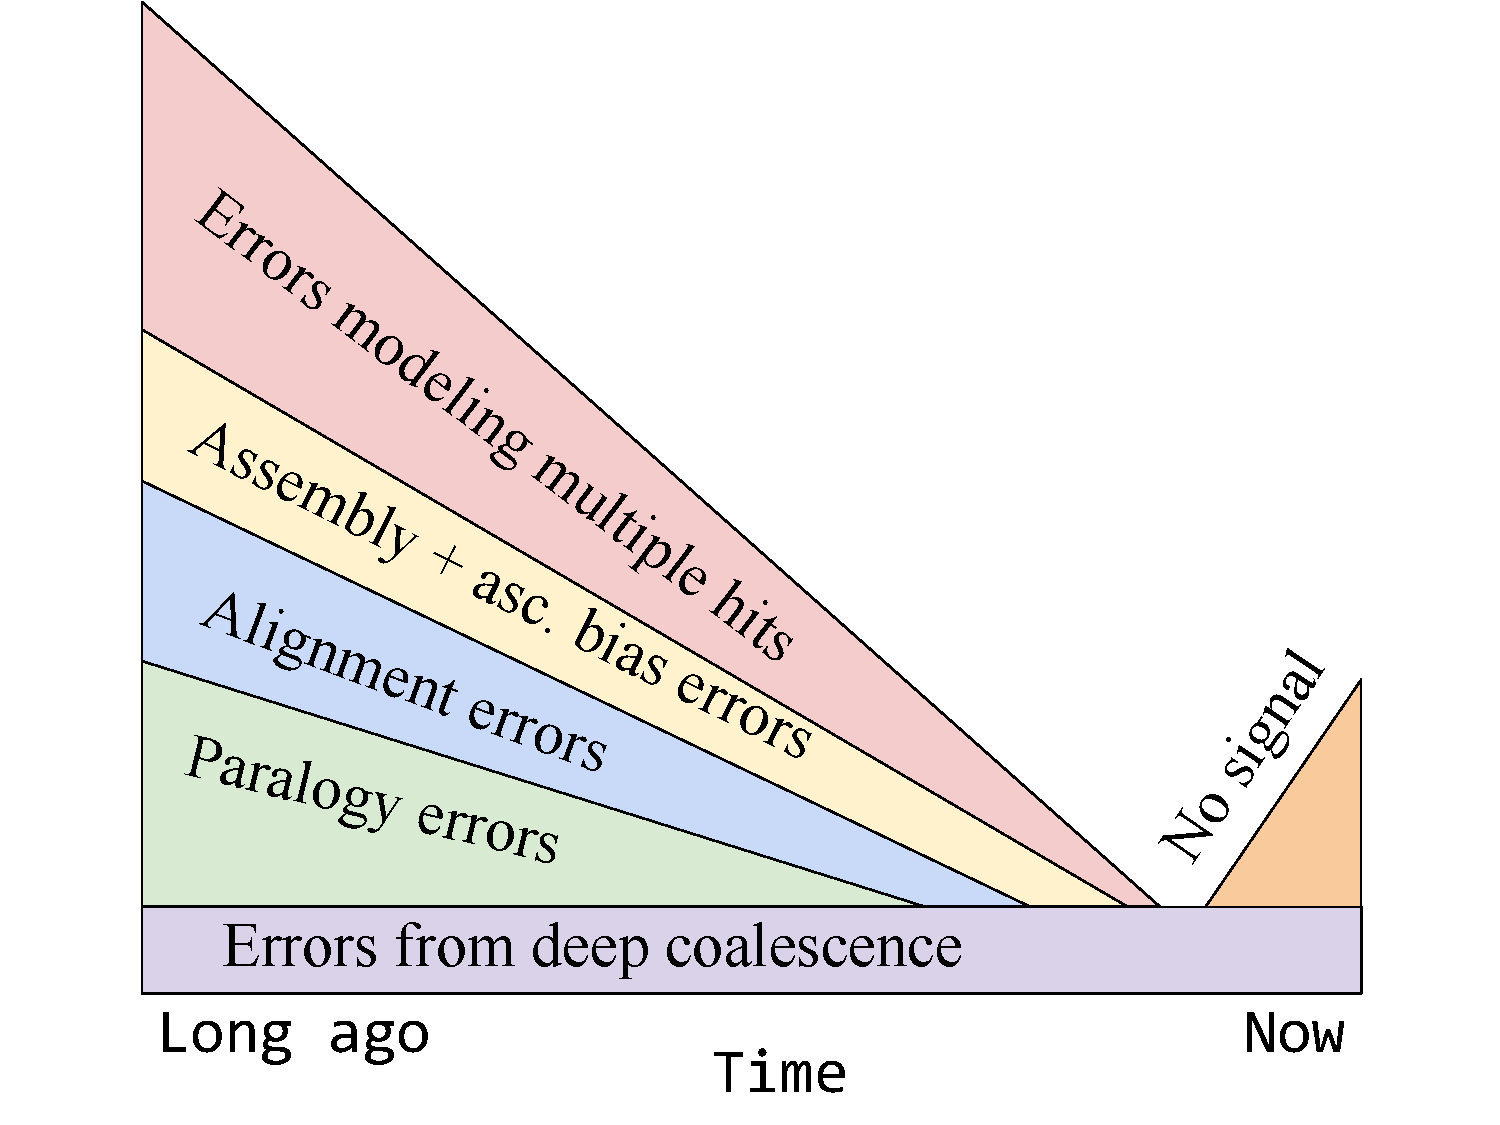
\includepdf[offset=0.0cm -1cm]{/home/mtholder/Documents/storage/talks/teaching/WoodsHole/testing/newimages/source-of-phylo-error-by-lookback-time.pdf}


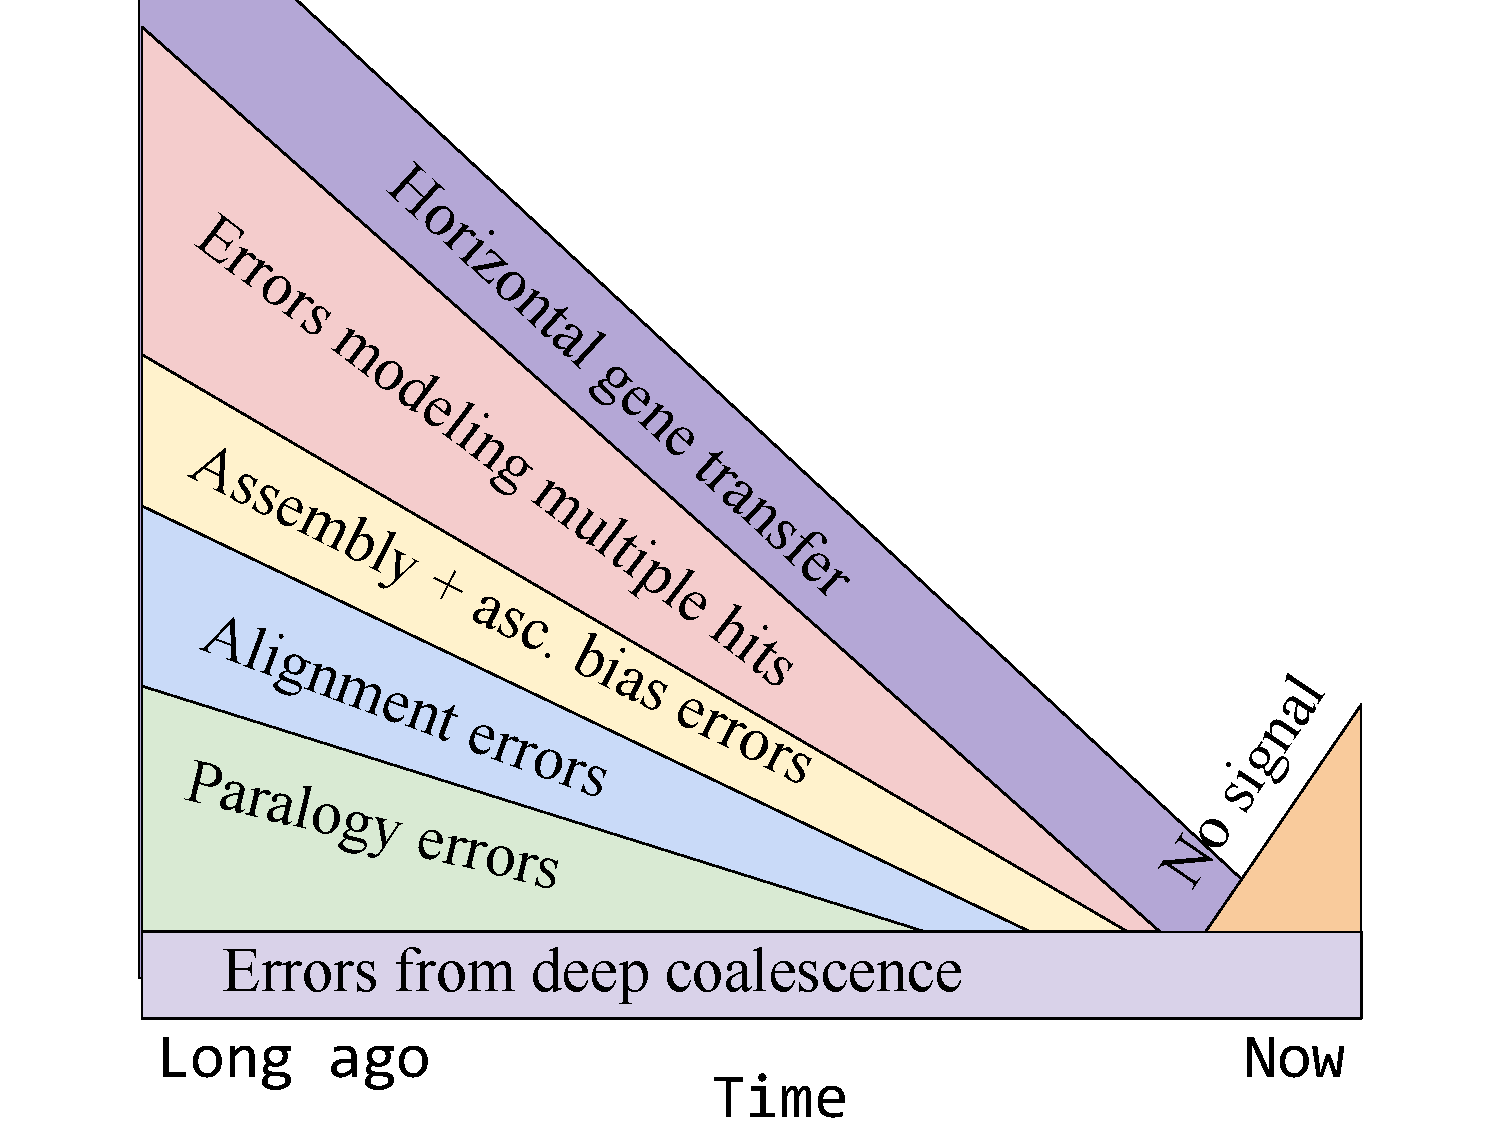
\includepdf[offset=0.0cm -1cm]{/home/mtholder/Documents/storage/talks/teaching/WoodsHole/testing/newimages/source-of-bact-phylo-error-by-lookback-time.pdf}


\myNewSlide
\section*{Tree and parameter sensitivity interact}
\footnotesize{From \citet{WrightEtAl2015}}\\
\begin{picture}(-0,0)(-0,0)
    \put(-70,-20){\makebox(30,-150)[l]{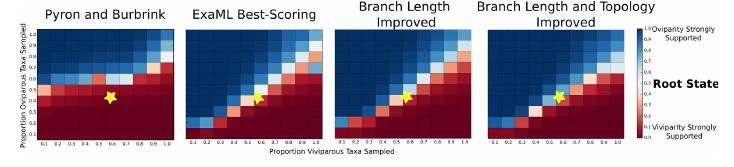
\includegraphics[scale=1.4]{/home/mtholder/Documents/storage/talks/teaching/WoodsHole/testing/newimages/WrightEtAl2015Fig4.jpeg}}}
    \put(50,-250){\makebox(30,-100)[l]{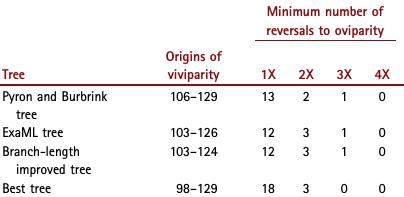
\includegraphics[scale=1.4]{/home/mtholder/Documents/storage/talks/teaching/WoodsHole/testing/newimages/WrightEtAl2015Table2.jpeg}}}
\end{picture}



